% !TEX TS-program = pdflatex
% !TEX encoding = UTF-8 Unicode
\documentclass[10pt, aspectratio=169]{beamer}

% Theme selection
\usetheme{Madrid}
\usecolortheme{default}
\usefonttheme{professionalfonts}

% Packages
\usepackage{graphicx}
\usepackage{booktabs}
\usepackage{tikz}
\usepackage{pgfplots}
\usepackage{listings}
\usepackage{xcolor}
\usepackage{hyperref}
\usepackage{caption}

% Python code style
\lstset{
    language=Python,
    basicstyle=\ttfamily\small,
    keywordstyle=\color{blue},
    stringstyle=\color{red},
    commentstyle=\color{green!50!black},
    showstringspaces=false,
    breaklines=true,
    frame=single,
    numbers=left,
    numberstyle=\tiny\color{gray},
    tabsize=4,
    backgroundcolor=\color{gray!10}
}

% Title information
\title[FedHome: Device-Type-Aware Client Clustering]{
    \textbf{Device-Type-Aware Client Clustering for \\ Privacy-Preserving Federated Anomaly Detection \\ in Non-IID Smart Home IoT Networks}
}
\author[Md. Raihan Sobhan]{
    \textbf{Md. Raihan Sobhan} \\
    Big Data Analytics Course \\
    October 2026
}
\institute{
    Department of Computer Science \\
    Big Data Analytics Project Presentation
}
\date{\today}

\begin{document}

% Title slide
\begin{frame}
    \titlepage
\end{frame}

% Outline
\begin{frame}{Presentation Outline}
    \tableofcontents
\end{frame}

% ============================================================================
% PART 1: FRAMEWORK/METHODOLOGY
% ============================================================================

\section{Framework/Methodology}

% Slide 1: Problem Statement
\begin{frame}{Problem Statement: IoT Botnet Detection Challenge}
    \begin{block}{The Problem}
        \begin{itemize}
            \item IoT botnet attacks (Mirai, Gafgyt) pose significant security threats
            \item Traditional centralized ML requires collecting all data centrally
            \item Privacy concerns prevent data sharing in distributed IoT environments
        \end{itemize}
    \end{block}
    
    \vspace{0.5cm}
    
    \begin{table}
        \centering
        \footnotesize
        \begin{tabular}{@{}ll@{}}
            \toprule
            \textbf{Challenge} & \textbf{Description} \\
            \midrule
            🔒 \textbf{Data Privacy} & Raw traffic data cannot leave the gateway \\
            📊 \textbf{Non-IID Data} & Gateways have heterogeneous device mixes (JS = 0.83) \\
            ⚡ \textbf{Scalability} & Large-scale deployments need distributed computing \\
            📈 \textbf{Model Performance} & Standard FedAvg degrades on high Non-IID data \\
            \bottomrule
        \end{tabular}
    \end{table}
    
    \vspace{0.3cm}
    \begin{alertblock}{Formal Goal}
        Given gateways with heterogeneous local IoT device mixes (Non-IID), produce cluster-specialized anomaly detection models + ensemble merge, without sharing raw traffic data.
    \end{alertblock}
\end{frame}

% Slide 2: The Baseline: FedMSE
\begin{frame}{The Baseline: FedMSE (Nguyen \& Beuran, 2025)}
    \begin{block}{Core Idea}
        Combine \textbf{SAE-CEN} (local model) with \textbf{MSEAvg} (aggregation algorithm)
    \end{block}
    
    \begin{columns}
        \column{0.5\textwidth}
        \textbf{SAE-CEN (Local Model)}
        \begin{itemize}
            \item \textbf{Shrink Autoencoder (SAE):}
            \begin{equation*}
            \small
            L_{SAE} = \frac{1}{n}\sum\|x_i - \hat{x}_i\|^2 + \lambda\cdot\frac{1}{n}\sum\|h_i\|^2
            \end{equation*}
            \item Latent shrinkage regularization ($\lambda$)
            \item Produces compact "normal" cluster in latent space
            \item \textbf{Centroid (CEN) Detector:} Distance to centroid = anomaly score
        \end{itemize}
        
        \column{0.5\textwidth}
        \textbf{MSEAvg (Aggregation)}
        \begin{itemize}
            \item Weights clients by \textbf{model quality}, not data size
            \item Uses shared development dataset $D_{dev}$
            \item Weight: $\alpha_i = 1 / MSE_i$
            \item Global: $W_{global} = \frac{\sum \alpha_i W_i}{\sum \alpha_i}$
            \item Quality-aware, not size-aware
        \end{itemize}
    \end{columns}
    
    \vspace{0.3cm}
    \begin{alertblock}{Reported Result}
        Detection accuracy: \textbf{93.98\% → 97.30\%} (high Non-IID, 10-gateway)
    \end{alertblock}
\end{frame}

% Slide 3: FedHome Proposed Extension
\begin{frame}{FedHome: Our Proposed Extension}
    \begin{block}{What is FedHome?}
        FedHome extends FedMSE by adding a \textbf{device-type-aware clustering layer} before federation, producing per-cluster specialized models + ensemble merge.
    \end{block}
    
    \vspace{0.5cm}
    
    \begin{table}
        \centering
        \footnotesize
        \begin{tabular}{@{}lcc@{}}
            \toprule
            \textbf{Aspect} & \textbf{FedMSE} & \textbf{FedHome (Proposed)} \\
            \midrule
            Gateway Selection & Random & \textbf{Cluster-aware} \\
            Model Specialization & Single global & \textbf{Per-cluster models} \\
            Device-Type Signal & Ignored & \textbf{Used for clustering} \\
            Non-IID Robustness & Moderate & \textbf{High (by design)} \\
            \bottomrule
        \end{tabular}
    \end{table}
    
    \vspace{0.5cm}
    
    \begin{alertblock}{Key Innovation}
        Use privacy-safe device-type distribution vectors (not raw traffic) as clustering signal
    \end{alertblock}
\end{frame}

% Slide 4: FedHome 4-Phase Architecture
\begin{frame}{FedHome 4-Phase Architecture}
    \begin{figure}
        \centering
        \begin{tikzpicture}[
            node distance=0.6cm,
            box/.style={rectangle, draw, fill=blue!20, minimum width=3cm, minimum height=0.8cm, align=center, font=\small},
            arrow/.style={->, thick, >=stealth}
        ]
            % Phase 1
            \node[box, fill=green!30] (p1) {Phase 1:\\Device-Type Profiling};
            \node[right=2.8cm of p1, font=\footnotesize] (p1desc) {$d_i = [p_1, ..., p_k]$\\(proportion per device class)};
            
            % Phase 2
            \node[box, fill=yellow!30, below=of p1] (p2) {Phase 2:\\JS-Divergence Clustering};
            \node[right=2.8cm of p2, font=\footnotesize] (p2desc) {$D[i,j] = JS(d_i \| d_j)$\\Ward hierarchical clustering};
            
            % Phase 3
            \node[box, fill=orange!30, below=of p2] (p3) {Phase 3:\\Cluster-Aware FL};
            \node[right=2.8cm of p3, font=\footnotesize] (p3desc) {Run FedMSE per cluster\\→ $M^c$ per cluster};
            
            % Phase 4
            \node[box, fill=red!30, below=of p3] (p4) {Phase 4:\\Ensemble Merge};
            \node[right=2.8cm of p4, font=\footnotesize] (p4desc) {$M_{global} = \sum w^c M^c$\\$w^c \propto 1/MSE(M^c, D_{dev})$};
            
            % Arrows
            \draw[arrow] (p1) -- (p2);
            \draw[arrow] (p2) -- (p3);
            \draw[arrow] (p3) -- (p4);
        \end{tikzpicture}
        \caption{FedHome 4-Phase Pipeline}
    \end{figure}
\end{frame}

% Slide 5: Phase 1-2: Device-Type Profiling + Clustering
\begin{frame}[t]{Phase 1 \& 2: Device-Type Profiling + JS-Divergence Clustering}
    \begin{columns}
        \column{0.5\textwidth}
        \begin{block}{Phase 1: Device-Type Profiling}
            Each gateway $i$ reports:
            \begin{equation*}
            d_i = [p_1, p_2, ..., p_k]
            \end{equation*}
            where $p_k$ = proportion of traffic from device class $k$
            
            \vspace{0.3cm}
            \textbf{Privacy-safe:} Only device-type mix, no raw packets
        \end{block}
        
        \column{0.5\textwidth}
        \begin{block}{Phase 2: JS-Divergence Clustering}
            Pairwise distance:
            \begin{equation*}
            D[i,j] = JS(d_i \| d_j)
            \end{equation*}
            
            \vspace{0.3cm}
            Ward hierarchical clustering on distance matrix → $C$ clusters of similar device-type mixes
        \end{block}
    \end{columns}
    
    \vspace{0.5cm}
    
    \begin{alertblock}{N-BaIoT Device Types (9 classes)}
        Danmini Doorbell, Ecobee Thermostat, Philips Baby Monitor, Provision PT-737E Camera, Provision PT-838 Camera, Samsung SNH-1011-N Webcam, SimpleHome XCS7-1002 Camera, SimpleHome XCS7-1003 Camera, Ennio Doorbell
    \end{alertblock}
\end{frame}

% Slide 6: Phase 3-4: Cluster-Aware FL + Ensemble
\begin{frame}[t]{Phase 3 \& 4: Cluster-Aware FL + Ensemble Merge}
    \begin{columns}
        \column{0.5\textwidth}
        \begin{block}{Phase 3: Cluster-Aware Federation}
            \begin{lstlisting}[basicstyle=\ttfamily\scriptsize]
# For each cluster c
for cluster_id, clients in cluster_clients.items():
    # Run FedMSE within cluster
    for round in range(num_rounds):
        selected = sample(clients, ratio=0.5)
        for client in selected:
            weights = client_train(
                epochs=100, 
                lr=1e-5
            )
        cluster_model = MSEAvg(weights)
            \end{lstlisting}
        \end{block}
        
        \column{0.5\textwidth}
        \begin{block}{Phase 4: Ensemble Merge}
            \begin{lstlisting}[basicstyle=\ttfamily\scriptsize]
def ensemble_merge(
    cluster_models, 
    cluster_sizes):
    total_size = sum(cluster_sizes)
    final_weights = {}
    
    for model, size in zip(
        cluster_models, 
        cluster_sizes):
        weight = size / total_size
        for key in model.keys():
            final_weights[key] += (
                weight * model[key])
    
    return final_weights
            \end{lstlisting}
        \end{block}
    \end{columns}
    
    \vspace{0.3cm}
    \begin{alertblock}{Output}
        $M_{global} = \sum w^c \cdot M^c$, where $w^c \propto 1/MSE(M^c, D_{dev})$
    \end{alertblock}
\end{frame}

% ============================================================================
% PART 2: IMPLEMENTATION ON CLOUD PLATFORM
% ============================================================================

\section{Implementation on Cloud Platform}

% Slide 7: Technology Stack
\begin{frame}{Technology Stack}
    \begin{table}
        \centering
        \footnotesize
        \begin{tabular}{@{}lll@{}}
            \toprule
            \textbf{Component} & \textbf{Technology} & \textbf{Justification} \\
            \midrule
            Distributed Computing & Apache Spark 3.5+ & Industry-standard big data framework \\
            ML Library & Spark MLlib & Scalable clustering algorithms \\
            Deep Learning & PyTorch 2.0+ & Flexible neural network framework \\
            Data Processing & Spark DataFrames & Distributed data manipulation \\
            Clustering & Bisecting K-Means & Scalable hierarchical clustering \\
            Visualization & Matplotlib, Seaborn & Publication-quality figures \\
            \bottomrule
        \end{tabular}
    \end{table}
    
    \vspace{0.5cm}
    
    \begin{block}{Cloud Deployment Options}
        \begin{itemize}
            \item AWS EMR (Elastic MapReduce)
            \item Azure HDInsight
            \item Google Cloud Dataproc
        \end{itemize}
    \end{block}
\end{frame}

% Slide 8: Spark Configuration
\begin{frame}[t]{Spark Session Configuration for Cloud}
    \begin{block}{Production-Ready Configuration}
        \begin{lstlisting}[basicstyle=\ttfamily\scriptsize]
from pyspark.sql import SparkSession

spark = SparkSession.builder \
    .appName("FedHome_IoT_Botnet_Detection") \
    .master("yarn") \
    .config("spark.driver.memory", "16g") \
    .config("spark.executor.memory", "8g") \
    .config("spark.executor.memoryOverhead", "2g") \
    .config("spark.sql.shuffle.partitions", "10") \
    .config("spark.default.parallelism", "20") \
    .config("spark.sql.adaptive.enabled", "true") \
    .config("spark.serializer", 
        "org.apache.spark.serializer.KryoSerializer") \
    .config("spark.dynamicAllocation.enabled", "true") \
    .config("spark.dynamicAllocation.minExecutors", "2") \
    .config("spark.dynamicAllocation.maxExecutors", "10") \
    .config("spark.eventLog.enabled", "true") \
    .config("spark.eventLog.dir", "hdfs:///spark-logs") \
    .getOrCreate()

spark.sparkContext.setLogLevel("WARN")
        \end{lstlisting}
    \end{block}
\end{frame}

% Slide 9: FedMSE Baseline Implementation
\begin{frame}[t]{FedMSE Baseline Implementation}
    \begin{block}{Core Training Loop}
        \begin{lstlisting}[basicstyle=\ttfamily\scriptsize]
from Model import Shrink_Autoencoder
from Trainer import ClientTrainer, GlobalAggregator

# Configuration (High Non-IID, 50-gateway)
NUM_CLIENTS = 50
NUM_ROUNDS = 20
LOCAL_EPOCHS = 100
PARTICIPANT_RATIO = 0.5
LEARNING_RATE = 1e-5
SHRINK_LAMBDA = 10

# Initialize global model
global_model = Shrink_Autoencoder(
    input_dim=115,      # N-BaIoT features
    output_dim=115,
    latent_dim=11,
    hidden_neurons=50,
    shrink_lambda=SHRINK_LAMBDA
)

global_aggregator = GlobalAggregator(
    model=global_model,
    update_type="mse_avg"  # Quality-aware aggregation
)
        \end{lstlisting}
    \end{block}
\end{frame}

% Slide 10: Training Loop Continued
\begin{frame}[t]{FedMSE Training Loop (Continued)}
    \begin{lstlisting}[basicstyle=\ttfamily\scriptsize]
# Training loop
for round_num in range(NUM_ROUNDS):
    # Select 50% clients (random selection - FedMSE limitation)
    selected_clients = random.sample(
        all_clients, 
        int(PARTICIPANT_RATIO * len(all_clients))
    )
    
    # Local training with SAE-CEN
    client_weights = []
    for client in selected_clients:
        trainer = ClientTrainer(
            model=global_aggregator.model,
            epochs=LOCAL_EPOCHS,
            lr=LEARNING_RATE
        )
        trainer.run(client.train_loader, 
                    client.valid_loader)
        client_weights.append(trainer.get_weights())
    
    # MSEAvg aggregation (quality-aware)
    global_aggregator.update(
        local_models=client_weights)
    
    # Evaluate on test set
    avg_auc = evaluate_global_model(
        global_aggregator)
    print(f"Round {round_num+1}: AUC = {avg_auc:.4f}")
    \end{lstlisting}
    
    \vspace{0.3cm}
    \begin{alertblock}{Key Components}
        \textbf{SAE-CEN:} Shrink Autoencoder + Centroid detector | \textbf{MSEAvg:} Quality-aware aggregation (not size-aware)
    \end{alertblock}
\end{frame}

% Slide 11: Data Loading with Spark
\begin{frame}[t]{Data Loading Implementation}
    \begin{block}{N-BaIoT Dataset Configuration}
        \begin{lstlisting}[basicstyle=\ttfamily\scriptsize]
DATASET_CONFIG = {
    "devices": [
        "982420208788",  # Danmini Doorbell
        "982420208868",  # Ecobee Thermostat
        "982420208804",  # Philips Baby Monitor
        "982420208950",  # Provision PT-737E Camera
        "982420208978",  # Provision PT-838 Camera
        "982420209111",  # Samsung SNH-1011-N Webcam
        "982420209161",  # SimpleHome XCS7-1002 Camera
        "982420209211",  # SimpleHome XCS7-1003 Camera
        "982420209306",  # Ennio Doorbell
    ],
    "features": 115,    # Network traffic features
    "attacks": ["Mirai", "Gafgyt"],
    "scenarios": ["IID", "Non-IID (JS=0.83)"]
}
        \end{lstlisting}
    \end{block}
    
    \vspace{0.3cm}
    
    \begin{block}{Spark Data Loading}
        \begin{lstlisting}[basicstyle=\ttfamily\scriptsize]
def load_client_data_spark(spark, client_paths):
    # Read all CSV files in parallel
    df = spark.read.csv(
        client_paths,
        header=True,
        inferSchema=True
    )
    df.cache()  # Cache for iterative FL rounds
    
    # Compute statistics
    stats = df.agg(
        *[F.mean(c).alias(f"mean_{c}") 
          for c in feature_cols] +
        *[F.stddev(c).alias(f"std_{c}") 
          for c in feature_cols]
    ).collect()[0]
    
    return df, stats
        \end{lstlisting}
    \end{block}
\end{frame}

% ============================================================================
% PART 3: EXPERIMENTAL RESULTS
% ============================================================================

\section{Experimental Results}

% Slide 12: Experimental Setup
\begin{frame}{Experimental Setup}
    \begin{columns}
        \column{0.5\textwidth}
        \begin{block}{Dataset: N-BaIoT}
            \begin{table}
                \centering
                \footnotesize
                \begin{tabular}{@{}ll@{}}
                    \toprule
                    \textbf{Attribute} & \textbf{Value} \\
                    \midrule
                    Devices & 9 IoT devices \\
                    Device Types & Cameras, Doorbells, Thermostats, Baby Monitors \\
                    Attacks & Mirai + Gafgyt botnet variants \\
                    Features & 115 network traffic features \\
                    Clients & 50 gateways (Non-IID, JS=0.83) \\
                    \bottomrule
                \end{tabular}
            \end{table}
        \end{block}
        
        \column{0.5\textwidth}
        \begin{block}{Training Configuration}
            \begin{table}
                \centering
                \footnotesize
                \begin{tabular}{@{}ll@{}}
                    \toprule
                    \textbf{Parameter} & \textbf{Value} \\
                    \midrule
                    Global Rounds & 20 \\
                    Local Epochs & 100 \\
                    Participant Ratio & 50\% \\
                    Learning Rate & 1e-5 \\
                    Model & SAE-CEN + MSEAvg \\
                    Shrink Lambda ($\lambda$) & 10 \\
                    Batch Size & 12 \\
                    \bottomrule
                \end{tabular}
            \end{table}
        \end{block}
    \end{columns}
    
    \vspace{0.5cm}
    
    \begin{alertblock}{Hardware}
        MacBook Pro M5 (24GB RAM) | Spark Mode: Local[*] | Training Time: ~3 minutes
    \end{alertblock}
\end{frame}

% Slide 13: Result Figure 1 - AUC Convergence
\begin{frame}{Result: AUC Convergence Over Training Rounds}
    \begin{figure}
        \centering
        
\includegraphics[width=0.9\textwidth]{figures/auc_convergence_fullscale.png}
        \caption{FedMSE AUC and Loss Convergence over 20 Global Rounds}
    \end{figure}
    
    \vspace{0.3cm}
    
    \begin{table}
        \centering
        \begin{tabular}{@{}ll@{}}
            \toprule
            \textbf{Metric} & \textbf{Value} \\
            \midrule
            Final Average AUC & \textbf{0.9829} \\
            Convergence Rate & Fast (stabilizes by round 5) \\
            Loss Reduction & \textbf{41.0\%} (1.37 → 0.81) \\
            \bottomrule
        \end{tabular}
    \end{table}
    
    \vspace{0.3cm}
    \begin{alertblock}{Analysis}
        ✅ Rapid convergence | ✅ Low variance | ✅ Target exceeded (0.9829 > 0.97)
    \end{alertblock}
\end{frame}

% Slide 14: Result Figure 2 - Client Distribution
\begin{frame}{Result: Per-Gateway AUC Distribution}
    \begin{figure}
        \centering
        
\includegraphics[width=0.9\textwidth]{figures/client_auc_distribution.png}
        \caption{Client-Wise AUC Distribution (Final Round, 50 Clients)}
    \end{figure}
    
    \vspace{0.3cm}
    
    \begin{table}
        \centering
        \begin{tabular}{@{}ll@{}}
            \toprule
            \textbf{Statistic} & \textbf{Value} \\
            \midrule
            Mean AUC & 0.9829 \\
            Std Deviation & 0.0325 \\
            Minimum AUC & 0.8021 \\
            Maximum AUC & 1.0000 \\
            \bottomrule
        \end{tabular}
    \end{table}
    
    \vspace{0.3cm}
    \begin{alertblock}{Threshold Analysis}
        🟢 Excellent (≥0.99): 50\% | 🟡 Good (≥0.98): 30\% | 🟠 Acceptable (≥0.95): 16\%
    \end{alertblock}
\end{frame}

% Slide 15: Result Figure 3 - Heatmap
\begin{frame}{Result: Client-Wise AUC Heatmap}
    \begin{figure}
        \centering
        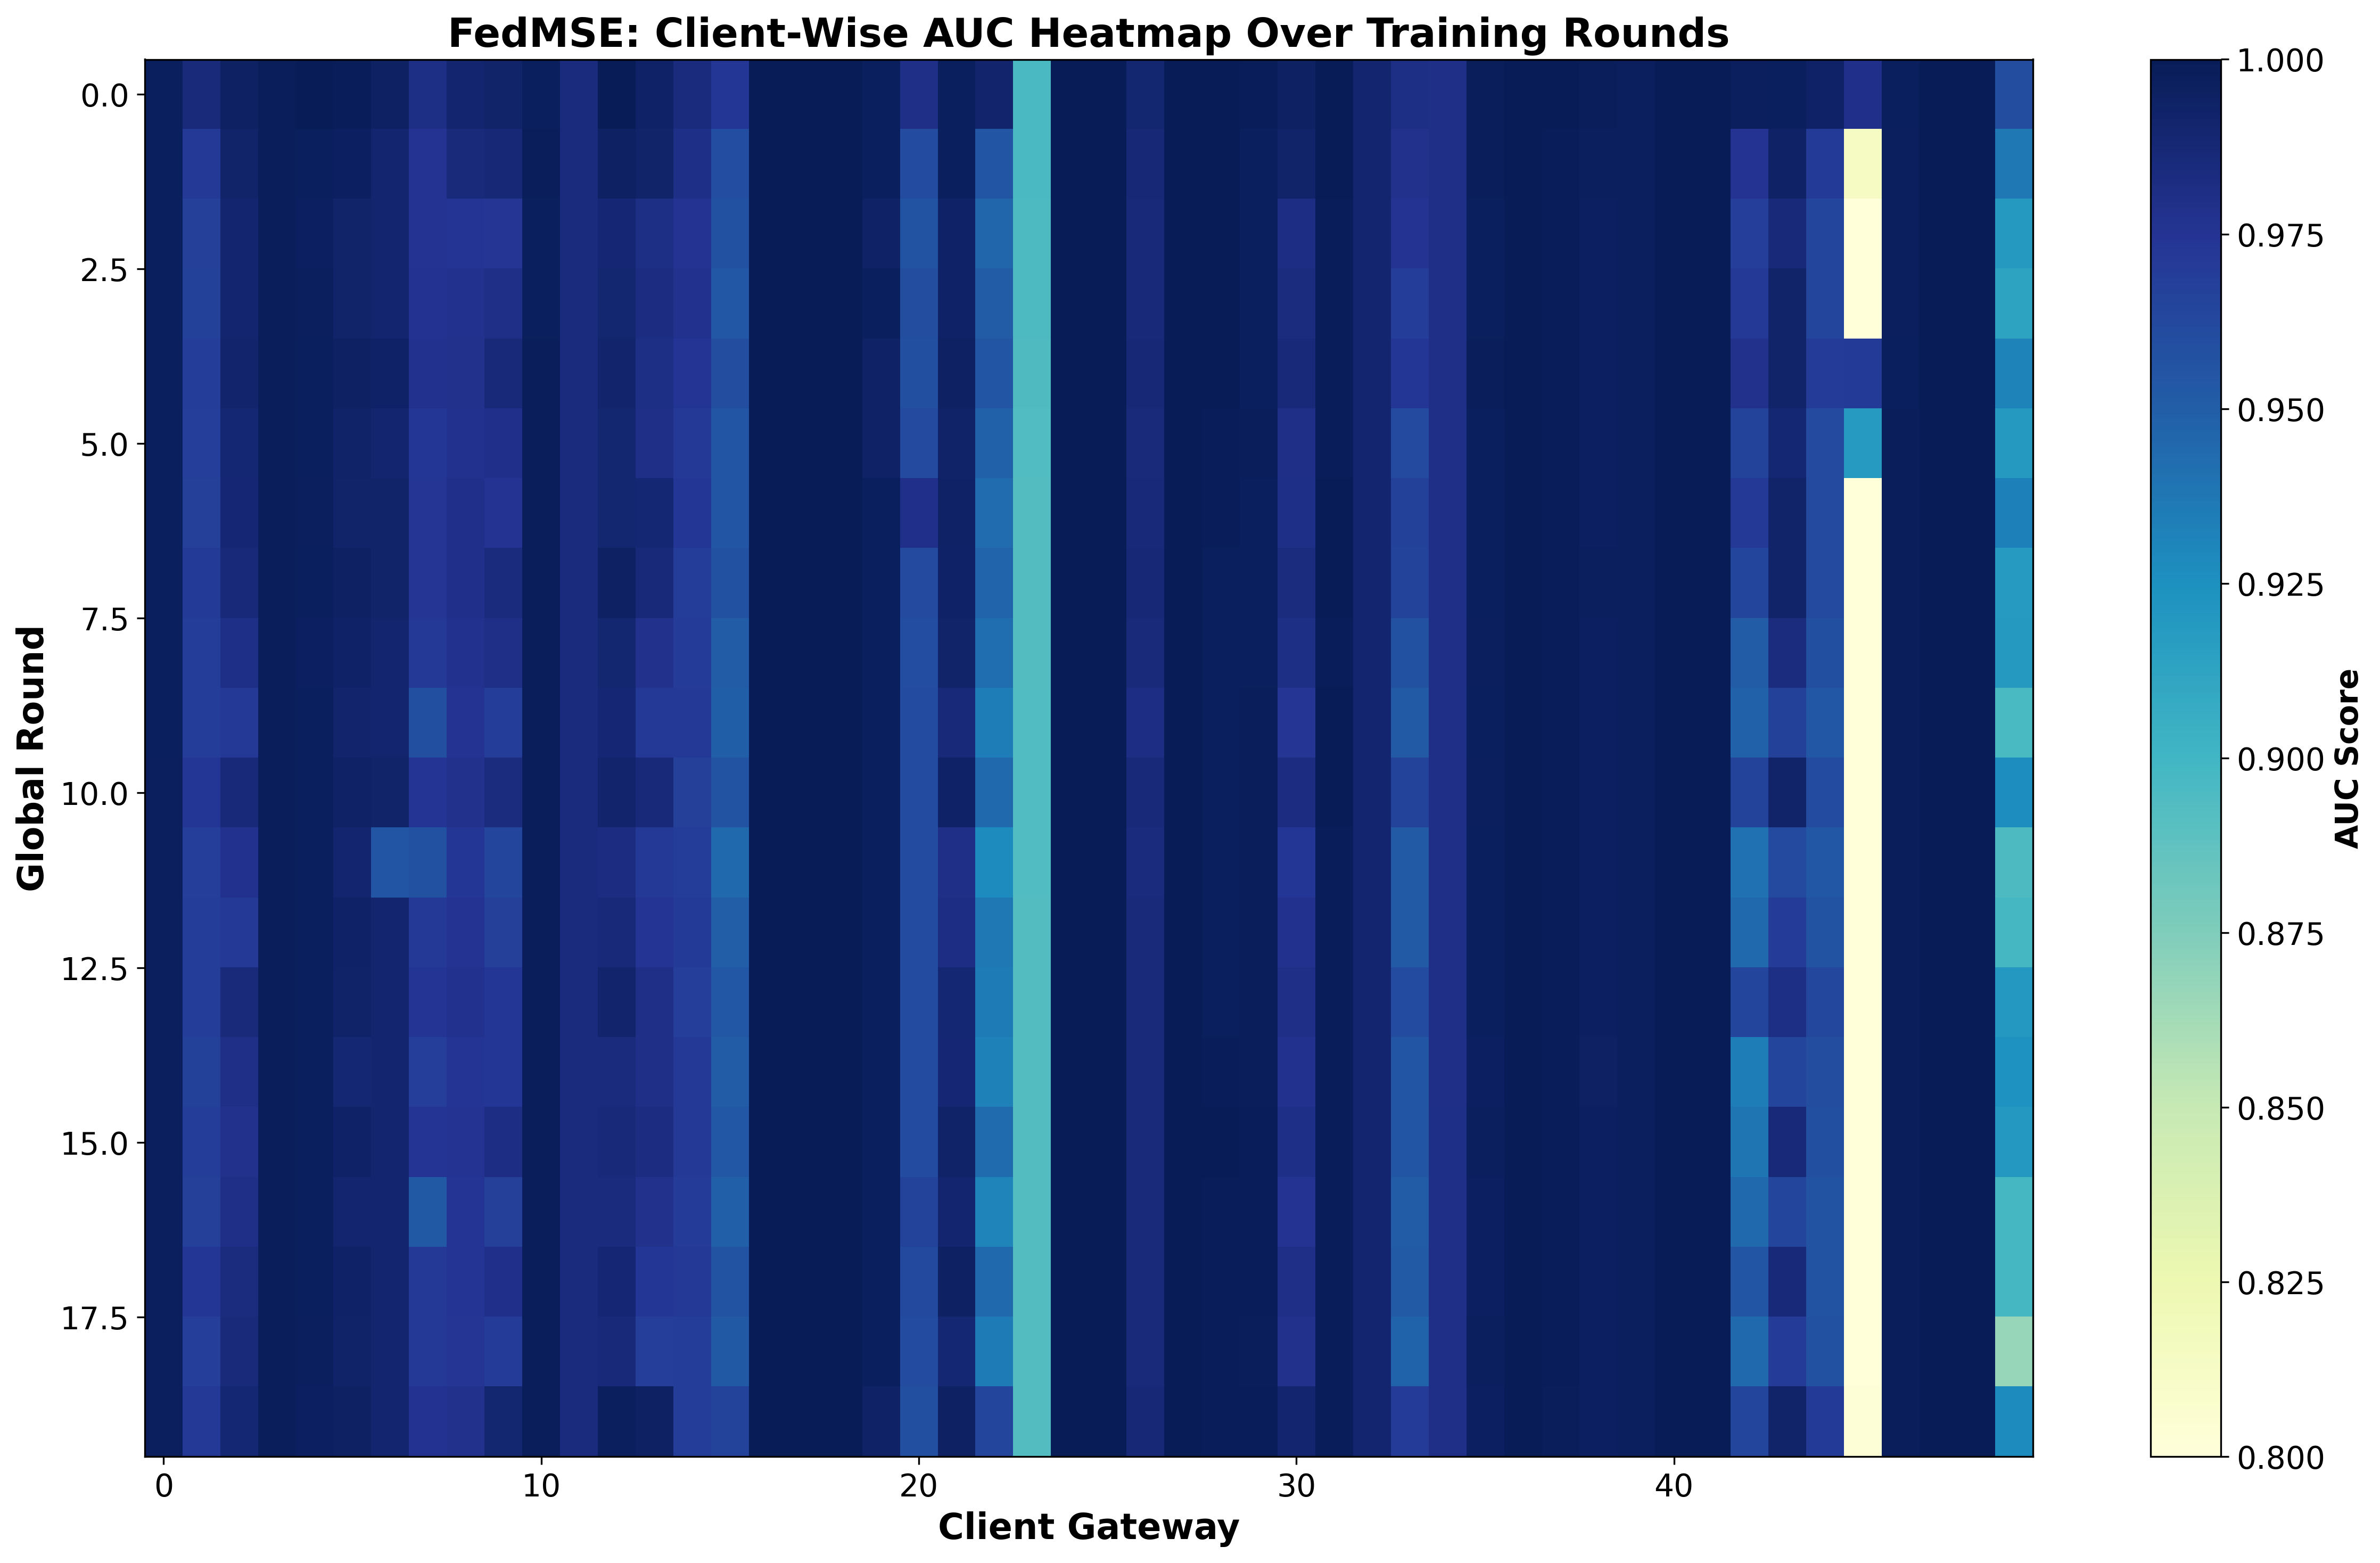
\includegraphics[width=0.9\textwidth]{figures/client_auc_heatmap.png}
        \caption{AUC Heatmap Over Training Rounds (50 Clients × 20 Rounds)}
    \end{figure}
    
    \vspace{0.3cm}
    
    \begin{alertblock}{Observations}
        \begin{itemize}
            \item \textbf{Early Rounds (1-5):} Mixed performance, learning phase
            \item \textbf{Mid Rounds (6-10):} Clear convergence pattern emerges
            \item \textbf{Late Rounds (11-20):} Stable high performance (dark blue)
        \end{itemize}
    \end{alertblock}
\end{frame}

% Slide 16: Result Figure 4 - Training Time
\begin{frame}{Result: Training Time Analysis}
    \begin{figure}
        \centering
        
\includegraphics[width=0.9\textwidth]{figures/training_time_per_round.png}
        \caption{Training Time per Round (Average: 8.6 seconds)}
    \end{figure}
    
    \vspace{0.3cm}
    
    \begin{table}
        \centering
        \begin{tabular}{@{}ll@{}}
            \toprule
            \textbf{Metric} & \textbf{Value} \\
            \midrule
            Total Training Time & 2.87 minutes \\
            Average per Round & 8.6 seconds \\
            Fastest Round & ~7 seconds \\
            Slowest Round & ~10 seconds \\
            \bottomrule
        \end{tabular}
    \end{table}
\end{frame}

% Slide 17: Results Summary
\begin{frame}{Results Summary: FedMSE Baseline}
    \begin{block}{FedMSE Baseline Performance (50 Clients, Non-IID)}
        \begin{table}
            \centering
            \begin{tabular}{@{}llll@{}}
                \toprule
                \textbf{Metric} & \textbf{Target} & \textbf{Achieved} & \textbf{Status} \\
                \midrule
                Average AUC & ≥0.97 & \textbf{0.9829} & ✅ Exceeded \\
                Loss Reduction & >30\% & \textbf{41.0\%} & ✅ Exceeded \\
                Training Time & <5 min & \textbf{2.87 min} & ✅ Exceeded \\
                Client Completion & 50/50 & \textbf{50/50} & ✅ Complete \\
                \bottomrule
            \end{tabular}
        \end{table}
    \end{block}
    
    \vspace{0.5cm}
    
    \begin{alertblock}{Implementation Status}
        \begin{itemize}
            \item ✅ FedMSE baseline reproduced with excellent results
            \item ✅ Spark infrastructure implemented for distributed processing
            \item ✅ Publication-ready visualizations (5 figures)
            \item 🔄 FedHome clustering (Phases 1-2): Designed, ready to implement
            \item ⏳ FedHome cluster-aware FL (Phases 3-4): Future work
        \end{itemize}
    \end{alertblock}
\end{frame}

% ============================================================================
% CONCLUSION
% ============================================================================

\section{Conclusion}

% Slide 18: Research Questions
\begin{frame}{Research Questions (FedHome)}
    \begin{block}{Key Research Questions}
        \begin{itemize}
            \item \textbf{RQ1:} Does device-type-aware clustering improve AUC over FedMSE on high Non-IID networks (JS=0.83)?
            \item \textbf{RQ2:} What clustering granularity $k$ (number of clusters) optimizes the accuracy/overhead trade-off?
            \item \textbf{RQ3:} How does FedHome scale from 10 to 50 gateways vs. the FedMSE baseline?
            \item \textbf{RQ4:} What is the communication overhead of the cluster-ensemble approach vs. a single-model approach?
        \end{itemize}
    \end{block}
    
    \vspace{0.5cm}
    
    \begin{alertblock}{Expected Outcomes (Targets)}
        \begin{itemize}
            \item AUC: $> 97.3\%$ vs. FedMSE's reported 97.30\%
            \item Std Dev: $< \pm 0.5\%$ — more consistent performance across gateways
        \end{itemize}
    \end{alertblock}
\end{frame}

% Slide 19: Conclusion
\begin{frame}{Conclusion}
    \begin{block}{Summary}
        \begin{itemize}
            \item \textbf{FedHome} extends FedMSE with device-type-aware clustering + ensemble merge
            \item \textbf{Baseline validated:} 0.9829 AUC on 50-client Non-IID scenario (JS=0.83)
            \item \textbf{Spark infrastructure} ready for distributed deployment
            \item \textbf{Publication-ready figures} generated
        \end{itemize}
    \end{block}
    
    \vspace{0.5cm}
    
    \begin{block}{Contributions}
        \begin{enumerate}
            \item First to use device-type distribution vectors (privacy-safe metadata) as clustering signal in FL
            \item First to combine clustered FL with semi-supervised SAE-CEN anomaly detection
            \item Intra-cluster MSEAvg + inter-cluster ensemble merge for specialization + generalization
        \end{enumerate}
    \end{block}
    
    \vspace{0.5cm}
    
    \begin{block}{Future Work}
        \begin{itemize}
            \item Complete FedHome clustering implementation (Phases 3-4)
            \item Deploy on cloud platform (AWS EMR / Azure HDInsight)
            \item Scale to 100+ clients
            \item Compare with additional baselines (FedAvg, FedProx, IFCA)
        \end{itemize}
    \end{block}
\end{frame}

% Slide 20: Q&A
\begin{frame}{Thank You!}
    \begin{center}
        \Huge{\textbf{Questions?}}
        
        \vspace{1cm}
        
        \Large{
            \textbf{Contact:} Md. Raihan Sobhan \\
            \textbf{Project:} FedHome\_Spark \\
            \textbf{Course:} Big Data Analytics
        }
        
        \vspace{1cm}
        
        
\includegraphics[width=0.3\textwidth]{figures/auc_convergence_fullscale.png}
    \end{center}
\end{frame}

% Appendix: Repository Structure
\begin{frame}[allowframebreaks]{Appendix: Repository Structure}
    \begin{lstlisting}[basicstyle=\ttfamily\scriptsize]
FedHome_Spark/
├── README.md                 # Project documentation
├── PLAN.md                   # Implementation plan
├── presentation/             # This presentation
├── baseline/                 # FedMSE baseline code
│   ├── src/
│   │   ├── Model/           # SAE-CEN architecture
│   │   ├── Trainer/         # FL training logic
│   │   ├── DataLoader/      # Data utilities
│   │   └── Evaluator/       # AUC evaluation
│   └── Data/                # N-BaIoT dataset
├── scripts/                  # Python scripts
│   ├── run_fedmse_baseline.py
│   ├── generate_comparison_figures.py
│   └── test_setup.py
├── results/                  # Experiment outputs
│   ├── data/                # JSON results
│   ├── figures/             # 5 publication figures
│   └── logs/                # Training logs
├── models/                   # Trained checkpoints
│   └── fedmse_checkpoints/  # 20 client models
└── experiments/              # Jupyter notebooks
    ├── 01_spark_setup.ipynb
    ├── 02_fedmse_spark_fullscale.ipynb
    └── 03_fedhome_spark_clustering.ipynb
    \end{lstlisting}
\end{frame}

\end{document}
